\chapter{Stato dell'Arte}
\section{Sistemi Ferroviari e Ferrotramviari}
Il concetto di \emph{treno} come comunemente percepito nasce con l'inizio della Rivoluzione Industriale, avvenuta tra il \emph{XVIII} e il \emph{XIX} secolo, a seguito della quale l'avvento della macchina a vapore ha permesso all'umanit\`a di disporre di fonti di energia sufficienti a fare evolvere i primi rudimentali trasporti su binario negli odierni sistemi ferroviari.\\*
\noindent\`E possibile schematizzare un Sistema Ferroviario, o Ferrotramviario, come un veicolo, il treno, vincolato a muoversi attraverso una propulsione, elettrica o a combustibile, lungo una traccia fissa, il binario.\\*
Queste caratteristiche accomunano qualsiasi sistema di trasporto ferroviario o ferrotramviario a prescindere dalla sua scala in termini di veicoli transitanti ed estensione geografica. Ci\'o che invece differenzia un Sistema Ferroviario da un Sistema Ferrotramviario sono:
\begin{itemize}
	\item Le caratteristiche fisiche del treno, come lunghezza e massa;
	\item Le caratteristiche geografiche dell'ambiente operativo;
	\item Gli scopi del trasporto.
\end{itemize}
In generale, nel trasporto ferroviario si utilizzano treni caratterizzati da grandi dimensioni, che trasportano persone o merci su lunghe percorrenze (regionali, nazionali o internazionali), operando pertanto prevalentemente in ambienti extra urbani. Un esempio di treno operante in un sistema ferroviario classico \`e quello in figura \ref{fig:frecciarossa}.\\*
\begin{figure}[h]
	\centering
	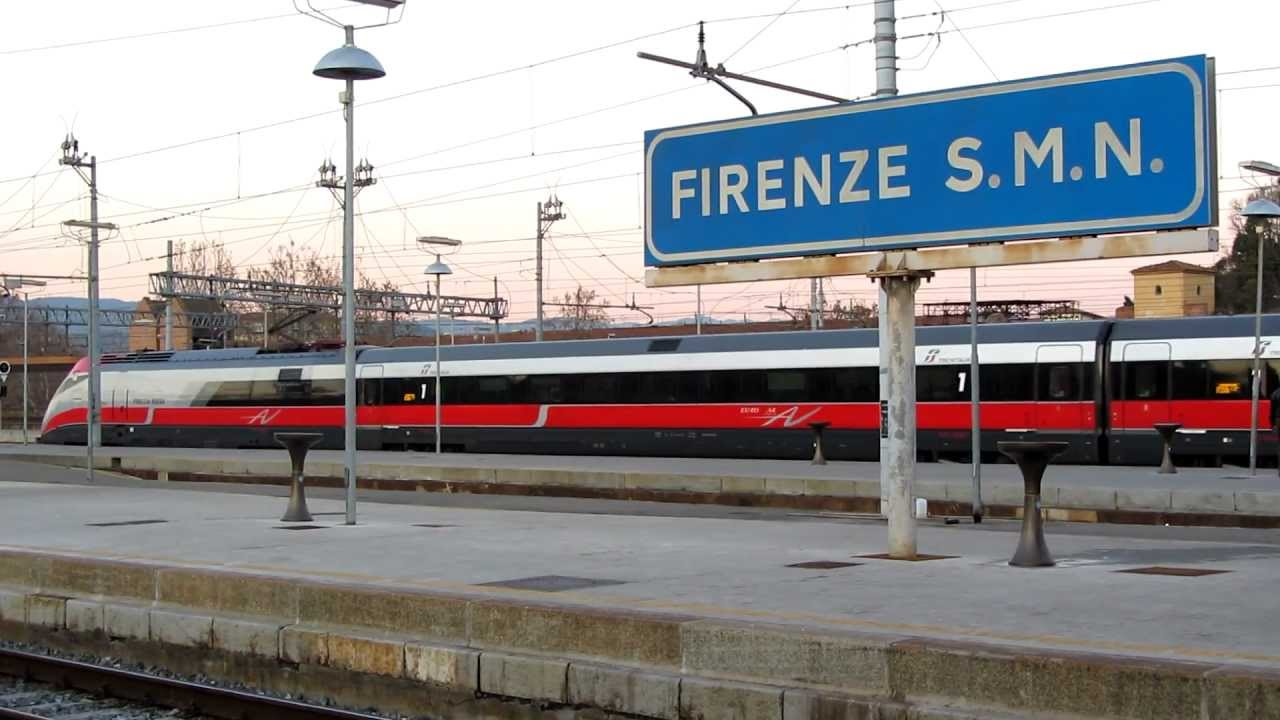
\includegraphics[width=0.7\linewidth]{img/frecciarossa}
	\caption{Treno in arrivo alla stazione ferroviaria di Firenze Santa Maria Novella}
	\label{fig:frecciarossa}
\end{figure}
Il trasporto ferrotramviario, di contro, vede l'utilizzo di treni dalle ridotte dimensioni, pi\'u leggeri di quelli usati nei sistemi ferroviari, e che hanno lo scopo di rappresentare un'alternativa per il cittadino all'utilizzo di mezzi privati durante i suoi spostamenti all'interno di un'area metropolitana. Quest'ultima caratteristica implica che l'ambiente operativo di un sistema ferrotramviario sia radicalmente diverso da quello di un sistema ferroviario: i treni si muovono lungo rotaie installate su strade urbane, quindi il traffico ferrotramviario \`e fuso con il traffico automobilistico, motociclistico, ciclistico e pedonale che caratterizza l'ambiente urbano, come mostrato nelle figure \ref{fig:danhai} e \ref{fig:tramschema}.\\*
\begin{figure}[h]
	\centering
	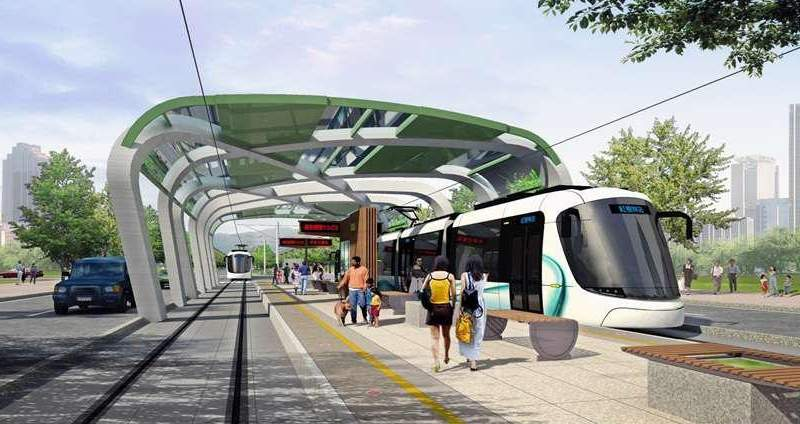
\includegraphics[width=0.7\linewidth]{img/danhai}
	\caption{Tramvia di Danhai, Taipan}
	\label{fig:danhai}
\end{figure}
\begin{figure}[h]
	\centering
	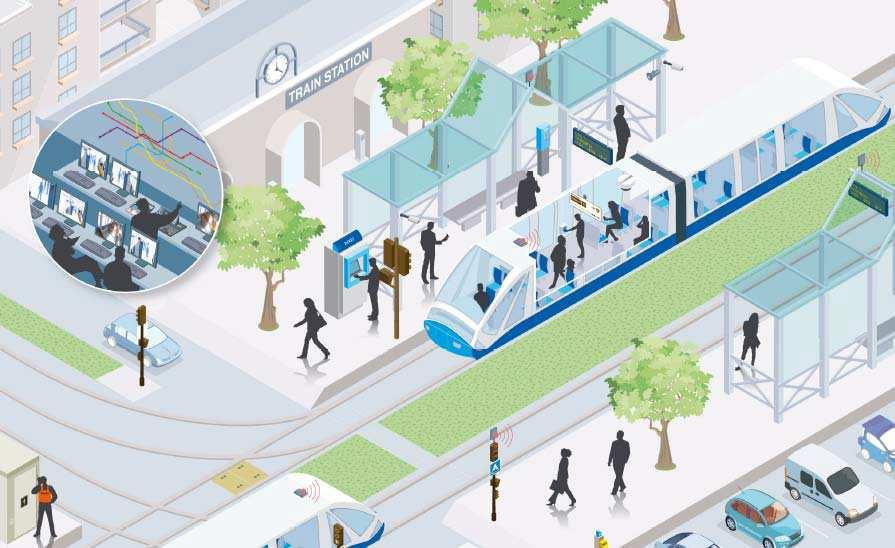
\includegraphics[width=0.7\linewidth]{img/twschema}
	\caption{Schema di un tipico scenario tramviario}
	\label{fig:tramschema}
\end{figure}
\subsection{Il Problema del Posizionamento}
Per posizionamento ferroviario, si intende la stima della posizione di un particolare treno all'interno di una particolare traccia ferroviaria. Spesso questa stima viene espressa come progressiva chilometrica rispetto all'origine della linea, oppure pi\'u raramente come coordinata geografica.\\*
Il problema del posizionamento sorge nel momento in cui, per ragioni di \emph{safety}, particolari sezioni di una traccia ferroviaria o ferrotramviaria, hanno caratteristiche tali da poter permettere il transito di un solo veicolo alla volta; basti pensare a una traccia 